\documentclass[twocolumn,superscriptaddress, prl,showpacs]{revtex4-1}
\setlength{\parskip}{0mm }
\setlength{\belowcaptionskip}{-10pt}
\usepackage{amsfonts}
\usepackage{amssymb}
\usepackage{amsmath}
\usepackage{amsthm}
\usepackage{dsfont}
\usepackage{graphicx}
\usepackage{stackrel}
\usepackage{color}

% Should come last b/c it needs to overload a bunch of commands
\usepackage{hyperref}

\newcommand{\ket}[1]{|#1\rangle}
\newcommand{\bra}[1]{\langle #1 |}
\newcommand{\be}{\begin{equation}}
\newcommand{\ee}{\end{equation}}



\begin{document}
\title{Supplementary Material}

\author{Hyungwon Kim}
\affiliation{Physics Department, Princeton University, Princeton, NJ 08544, USA}
\affiliation{Department of Physics and Astronomy, Rutgers University, Piscataway, NJ 08854, USA}

\author{Mari Carmen Ba\~{n}uls}
\affiliation{Max-Planck-Institut f$ {\ddot{u}}$r Quantenoptik, Hans-Kopfermann-Str. 1, 85748 Garching, Germany}

\author{J. Ignacio Cirac}
\affiliation{Max-Planck-Institut f$ {\ddot{u}}$r Quantenoptik, Hans-Kopfermann-Str. 1, 85748 Garching, Germany}

\author{Matthew B. Hastings}
\affiliation{Station Q, Microsoft Research, Santa Barbara, CA 93106-6105, USA}
\affiliation{Quantum Architectures and Computation Group, Microsoft Research, Redmond, WA 98052, USA}

\author{David A. Huse}
\affiliation{Physics Department, Princeton University, Princeton, NJ 08544, USA}
\begin{abstract}

\end{abstract}

\maketitle

\section{Operator Norm}
In the main text, we have used the square of the Frobenius norm to quantify the commutator with the Hamiltonian
and related it to the time scale of thermalization of the local operator.
In this section, we use the operator norm (the largest eigenvalue in magnitude),
to estimate the thermalization time scale.


Let us assume that $\hat{A}_M$ satisfies the following:
\begin{align}
||[\hat{A}_M, H]|| \leq \chi(M),
\end{align}
where $H$ is the Hamiltonian and $||\ldots||$ means the operator norm of the argument and $\chi(M)$ is some nonnegative valued function.
Then, using the Heisenberg equation of motion, we have
\begin{align}
\bigg|\bigg|\frac{d}{dt} \hat{A}_M(t)\bigg|\bigg| &= \bigg|\bigg| e^{-i H t} \left(\frac{d}{dt} \hat{A}_M (t)\right) e^{i H t} \bigg|\bigg| \nonumber\\
&= ||[\hat{A}_M(t = 0), H]|| \leq \chi(M) \\
||\hat{A}_M(t) - \hat{A}_M(0)|| &= \bigg|\bigg|\int_0^t \left(\frac{d}{d\tau} \hat{A}_M(\tau)\right)d\tau \bigg|\bigg| \nonumber\\
&\leq \int^t_0 \big|\big|\frac{d}{d\tau} \hat{A}_M(\tau)\big|\big|d\tau \leq \chi(M) t ~,
\end{align}
where we have used the fact that $e^{-iHt}$ is a norm-preserving unitary operator.
This inequality bounds the distance of an operator evolving under Hamiltonian dynamics
from its initial configuration. Next, we consider an initial state $\rho$ such that
\begin{align}
|\langle \hat{A}_M \rangle_0 - \langle \hat{A}_M \rangle_\beta| = \gamma(M) ~,
\end{align}
where $\langle \ldots \rangle_0$ is the expectation value of the initial condition, $\langle \ldots \rangle_\beta$
is thermal expectation value and $\gamma(M)$ is some nonnegative valued function.
Now we can estimate the distance between the thermal expectation value and the expectation value at time $t$ (for $t \leq \gamma(M)/\chi(M)$):
\begin{align}
&|\langle \hat{A}_M \rangle_t - \langle \hat{A}_M \rangle_\beta| \nonumber\\
&\geq \left | |\langle \hat{A}_M\rangle_0 - \langle \hat{A}_M\rangle_\beta | -|\langle \hat{A}_M\rangle_t - \langle \hat{A}_M\rangle_0 |\right | \nonumber\\
&\geq \gamma(M) - t \chi(M)
\end{align}
where $\langle \ldots \rangle_t$ is the expectation value at time $t$.
Therefore, if we have a sequence of $M$-body operators $\{ \hat{A}_M \}$
for which the operator norm of the commutator with the Hamiltonian decays fast with $M$
and an initial state which does not allow fast decrease of $\gamma(M)$,
the time scale of thermalization of $\hat{A}_M$ is
\begin{align}
\tau_M \sim \frac{\gamma(M)}{\chi(M)} ~,
\end{align}
which is an increasing function of $M$. 
In particular, if $\chi(M)$ decreases faster than a power law with $M$,
thermalization may take longer than polynomial time in the case of diffusion.



\begin{figure}
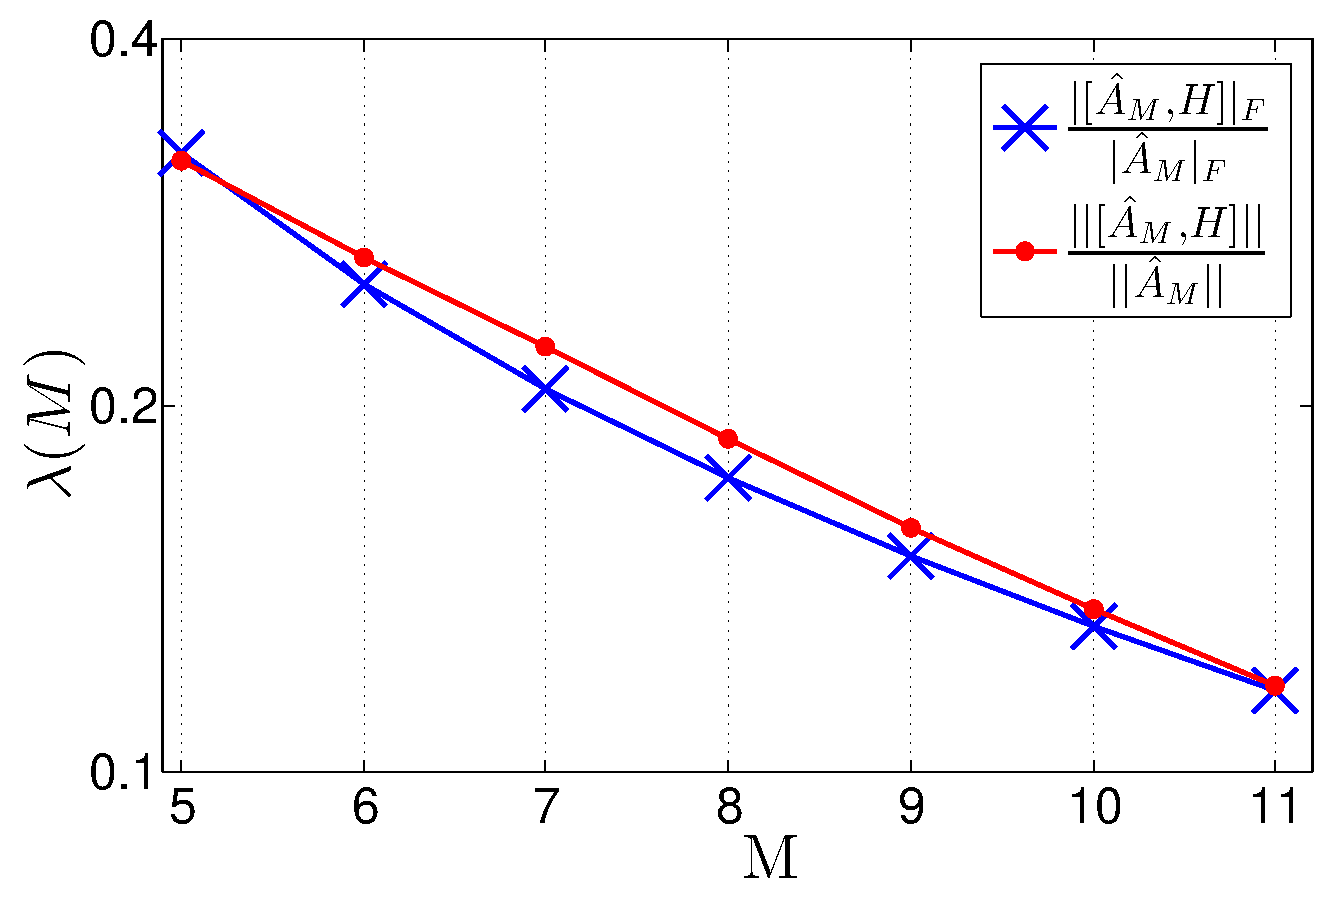
\includegraphics[width=1.0\linewidth]{infinite_ham_opnorm.pdf}
\centering
\caption{(color online) Normalized magnitude of $[\hat{A}_M, H]$ measured by the Frobenius norm ($|\ldots|_F$) and the operator norm ($||\ldots||$)
in log-linear plot.
$\hat{A}_M$ is obtained by minimizing the Frobenius norm of the commutator with Hamiltonian as is in the main text.
Two norms give quantitatively similar values.
}
\label{fig:op_norm}
\end{figure}

Mathematically, the operator norm is more convenient
since we can directly interpret the relaxation of the operator in terms of Lieb-Robinson bounds \cite{Lieb:1972,Bravyi:2006}.
Optimizing the operator norm numerically is, however, very challenging. Therefore, we used the (square of) Frobenius norm in the main text 
and related it with the time scale for a particular initial state, $\rho = I/Z + \epsilon \hat{A}_M$. 
Nevertheless, once we have an operator, it is easy to compute the operator norm of the commutator with Hamiltonian.
Figure \ref{fig:op_norm} plots the decay of the Frobenius norm and the operator norm of $[\hat{A}_M,H]$,
where $\hat{A}_M$ is obtained in the main text by minimizing the Frobenius norm.
It shows that the value of $\lambda$ measured by the operator norm is numerically similar to that of the Frobenius norm 
for the range of $M$ we studied.
It appears that the operator norms computed for these operators exhibit exponential-like decrease with $M$ but
the range of $M$ is not enough to draw a reliable conclusion.


\section{Results of another set of parameters}
\begin{figure}
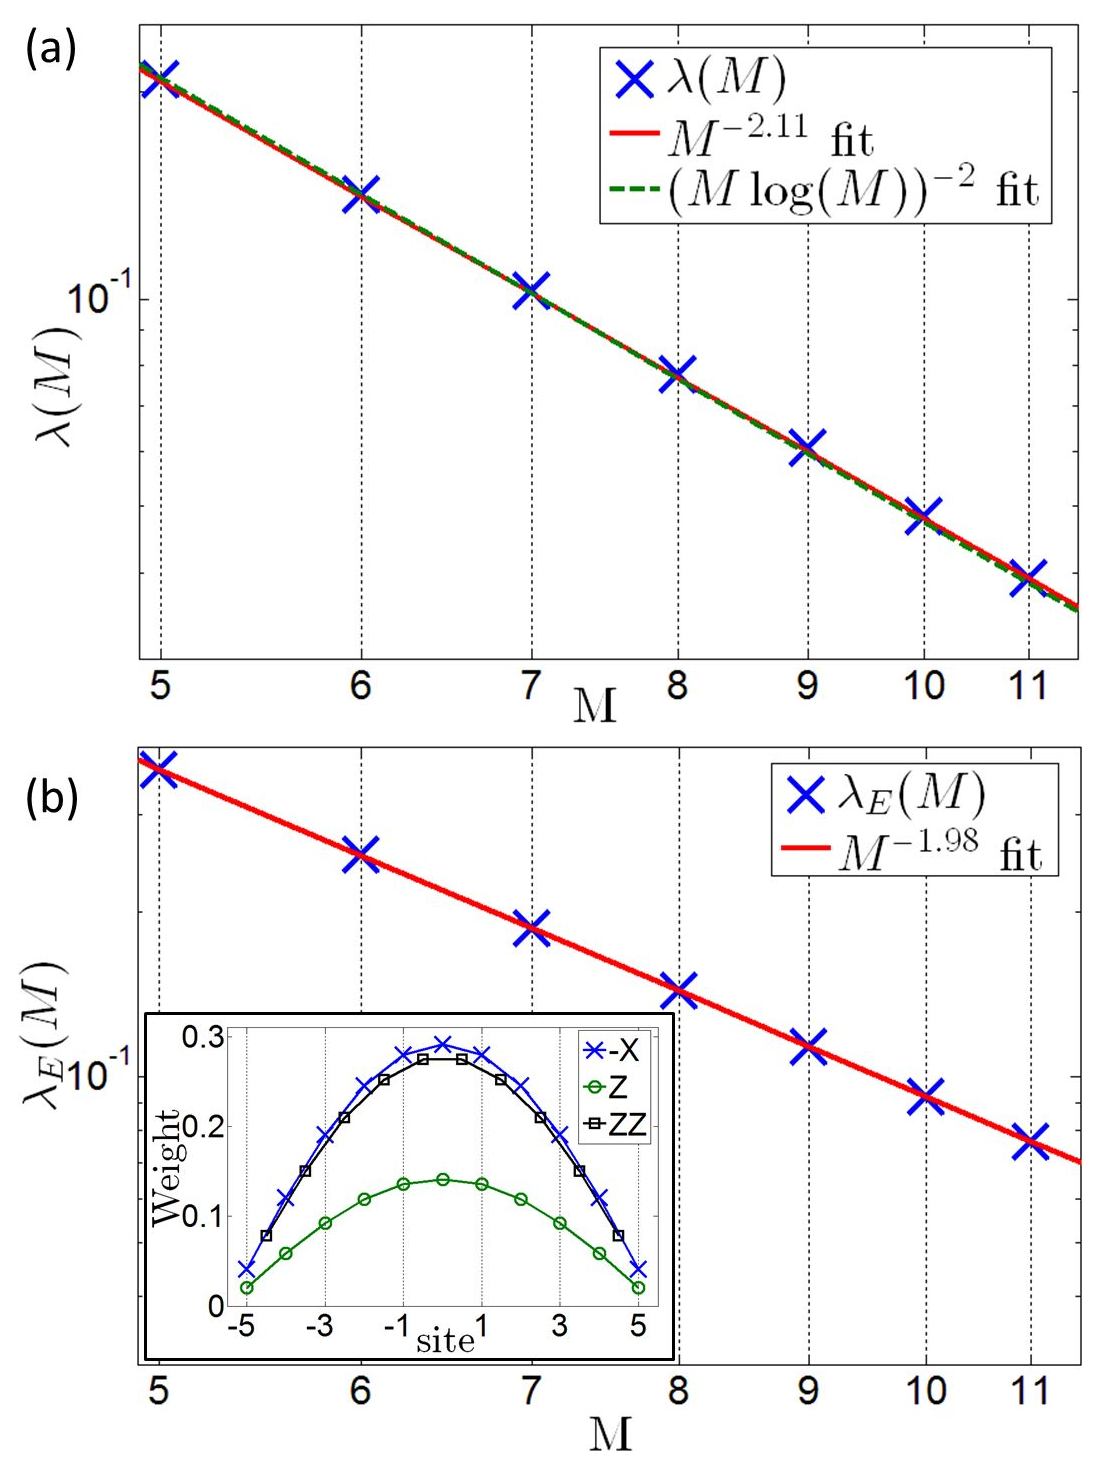
\includegraphics[width=1.0\linewidth]{fig_hamiltonian_other.pdf}
\centering
\caption{(color online) (a) $\lambda(M)$ is the minimum value of the Frobenius norm of the commutator with Hamiltonian.
Here we choose the parameters to be $(g,h) = (-1.05, 0.5)$. $\lambda$ still decreases faster than $1/M^2$.
(b) $\lambda_E(M)$ is the same results when we restrict the search space within the terms in the Hamiltonian.
As expected, it has $M^{-2}$ scaling and the structure is cosine modulation (inset).}
\label{fig:hamiltonian_other}
\end{figure}
In this section, we show that the results in the main body do not depend on the parameter choice.
We choose another set of parameters $(g,h) = (-1.05, 0.5)$, which is the parameter choice of Ref.~\onlinecite{Banuls:2011}.

Figure \ref{fig:hamiltonian_other} (a) is the minimum value of $f(\hat{A}_M)$ (Eqs. (3) and (4) in the main text) with the other parameter choice.
We can see that it decays faster than $1/M^2$. As is the case of the parameter choice in the main text,
the data can be well-fitted by two methods; a power-law and a logarithmic correction to $1/M^2$.
Since the power-law exponent could depend on the parameter choice, we do not attempt to draw a strong conclusion from this data
except that $\lambda(M)$ decreases faster than $1/M^2$,
the scaling of the diffusive energy mode.

Figure \ref{fig:hamiltonian_other} (b) is the plot of $\lambda_E(M)$ (minimized by only using terms in Hamiltonian)
for $(g,h) = (-1.05, 0.5)$. Unlike the case where all operators are used,
the decay scaling remains the same as $1/M^2$ as expected from the hydrodynamics.
Therefore, we again explicitly demonstrate that the longest wavelength energy modulation is the slowest mode of a conserved quantity.


\section{Slow Operators for Arbitrary Quantum Circuits}
We now show that a slowly relaxing operator must always exist, on an interval of length $M$ with the relaxation rate going to zero as $M$ gets large.  Let $U$ be the unitary of the quantum circuit restricted to an interval of length slightly larger than $M$ (in this way, we can consider only finite dimensional spaces).

Let ${\cal E}(\hat{O})$ be a super-operator defined by ${\cal E}(\hat{O})=U\hat{O}U^\dagger$.  The space of operators can be regarded as a vector space, with inner product $(A,B)={\rm tr}(A^\dagger B)$, and with ${\cal E}(\hat{O})$ being a linear operator on this space.  The operator ${\cal E}$ is non-Hermitian but it is a normal operator, since its Hermitian conjugate is equal to ${\cal E}^\dagger(\hat{O})=U^\dagger \hat{O} U$ and ${\cal E}({\cal E}^\dagger(\hat{O}))={\cal E}^\dagger({\cal E}(\hat{O}))=\hat{O}$ and so $[{\cal E},{\cal E}^\dagger]=0$.
Let ${\cal E}_h=\frac{1}{2}({\cal E}+{\cal E}^\dagger)$ and ${\cal E}_a=\frac{1}{2i}({\cal E}-{\cal E}^\dagger)$.

We begin by constructing an operator $\hat{O}$ supported on an interval of length $M$ such that ${\cal E}_h(\hat{O})= x \hat{O}+\hat{\epsilon}$ for some $x$ and for $\hat{\epsilon}={\cal O}(1/M)$.  Let $A$ be any traceless operator supported on a single site in the center of the interval.  We consider the Krylov space generated by the vectors $A, {\cal E}_h(A), {\cal E}_h^2(A),...$.  Let $K$ be the number of vectors we take; $K$ will be proportional to $M$ and will be chosen such that all these operators are supported on the interval of length $M$.
Since ${\cal E}_h$ is Hermitian, using the Lanczos procedure we can write it as a tridiagonal matrix $T$ in this Krylov space.   We claim that that there exists a vector $v$ supported on the first $K-1$ vectors $w_1,...,w_{K-1}$ such that $|Tv-xv|^2/|v|^2\leq {\cal O}(1/K^2)$.  To verify this claim, let $\psi$ be any eigenvector of $T$ with at least half its weight on the first $K/2$ vectors with $\psi=\sum_k a_k v_k$; let $x$ be the corresponding eigenvalue; let $v=\sum_k a_k (1-k/K) v_k$.
The basis in which the matrix is tridiagonal has basis vectors $w_1,w_2,...$, with $w_k$ being in the span of the first $k$ vectors $A, {\cal E}_h(A),...$
Hence, the vector $v$ gives us the desired operator $\hat{O}$.

Now consider the operators
\be
\hat{O}_{\pm}=(\sqrt{1-x^2} \pm {\cal E}_a) \hat{O},
\ee
with $\hat{O}$ normalized such that $||\hat{O}||=1$.
Note that ${\cal E}(\hat{O}_{\pm})={\cal E}_h(\hat{O}_{\pm})+i {\cal E}_a(\hat{O}_{\pm})=x\hat{O}_{\pm}+i(\sqrt{1-x^2}{\cal E}_a \pm {\cal E}_a^2) \hat{O} + {\cal O}(1/M)$.  Using
the fact that ${\cal E}_h^2+{\cal E}_a^2$ is equal to the identity super-operator, $(\sqrt{1-x^2}{\cal E}_a \pm {\cal E}_a^2) \hat{O}=\sqrt{1-x^2}{\cal E}_a \pm (1-x^2) ) \hat{O} +{\cal O}(1/M)=\pm\sqrt{1-x^2}\hat{O}_{\pm}+{\cal O}(1/M)$.
Hence,
\be
{\cal E}(\hat{O}_{\pm})=z \hat{O}_{\pm}+{\cal O}(1/M)
\ee
with
\be
z=x\pm i \sqrt{1-x^2},
\ee
so that $|z|=1$.
At least one of the two operators $\hat{O}_{\pm}$ must have non-negligible norm.  Let $X$ be the corresponding operator, normalized to have norm $1$.  Hence, we have constructed an operator $X$ supported on the interval of length $M$ such that ${\cal E}(X)=z X + {\cal O}(1/M)$.

This already implies that there is some operator $X$ which is slowly relaxing but perhaps oscillating; i.e., since $X$ is an approximate eigenoperator of ${\cal E}$, if $z=1$ then $X$ changes slowly over time, while if $z \neq 1$, then the expectation value of $X$ oscillates.

In fact, we can always construct an operator $Y$ which is an approximate eigenoperator of ${\cal E}$.  Here is one way.  Consider many disjoint intervals of length $M$.  Let $X_1,X_2,...$ be the operators on these intervals with eigenvalues $z_1,z_2,...$  Choose some subset $S$ of these intervals such that the product of the $z_i$ on that subset is close to $1$: $\prod_{i \in S} z_i \approx 1$.  Then, let $Y=\prod_{i \in S} X_i$.  This requires some analytic estimates to determine the support of $Y$ required: since $Y$ is a product of many operators, the error (in that each $X_i$ is only an approximate eigenoperator) may add, so the support of $Y$ may scale as a fairly large polynomial in the error.  We leave this estimate for later.

\section{$1/M^2$ scaling of filtered operators}
We show $1/M^2$ scaling of filtered operators of the form (Eq. (17) in the main text) if $\mathrm{tr}(\hat{O}U^n \hat{O}U^{-n}) = 0$ for all $n\neq 0$,
where $\hat{O}$ is a traceless Hermitian acting on a single site.
\begin{widetext}
First, observe that
\begin{align}
\frac{\mathrm{tr}([\tilde{A}_N,U][\tilde{A}_N,U])}{\mathrm{tr}(\tilde{A}_N\tilde{A}_N^\dag)} 
=2 - \bigg(\sum_{n,m = -N}^{N}c_n c_m \mathrm{tr}(U^{n-m-1}\hat{O}U^{-n+m+1}\hat{O} 
+ U^{n-m+1}\hat{O}U^{-n+m-1}\hat{O})\bigg)/\mathrm{tr}(\tilde{A}_N\tilde{A}_N^\dag) ~.
\end{align}
Therefore, if $\mathrm{tr}(\hat{O}U^n \hat{O}U^{-n}) = \delta_{n,0}\mathrm{tr}(\hat{O}\hat{O}^\dag)$,
the above expression simplifies to
\begin{align}
\frac{\mathrm{tr}([\tilde{A}_N,U][\tilde{A}_N,U])}{\mathrm{tr}(\tilde{A}_N\tilde{A}_N^\dag)}=2\left(1 - \frac{\sum_{n=-N}^{N-1}c_n c_{n+1}}{\sum_{n=-N}^N c_n^2}\right) ~.
\end{align}
This is a trivial quadratic optimization problem and the solution is $c_n = \cos(n\pi/(2N+2))$.
Therefore, the minimum value $\tilde{\lambda}$ for sufficiently large $N$ is
\begin{align}
\tilde{\lambda} &= \mathrm{min}\left[\frac{\mathrm{tr}([\tilde{A}_N,U][\tilde{A}_N,U])}{\mathrm{tr}(\tilde{A}_N\tilde{A}_N^\dag)} \right] = 2 - 2\cos\left(\frac{\pi}{2N+2}\right) \simeq \frac{\pi^2}{4(N+1)^2} \sim \frac{1}{M^2} ~,
\end{align}
where we used the fact that the support $M = 4N +1 $.
\end{widetext}

Ref. ~\onlinecite{Kim_ETH} has shown that the $U_F = e^{-i H_x \tau} e^{-i H_z \tau}$ (Eq. (12) in the main text) thermalizes a local operator at infinite temperature,
and thus $\mathrm{tr}(\hat{O}U^n\hat{O}U^{-n}) = 0$ for a sufficiently large $n$.
For the Floquet system, therefore, the above condition is approximately satisfied for a large enough $N$.
Figure 2 (b) in the main text shows that for $N$ = 60 and 100, the form is very close to the cosine
and the scaling for large $M = 2N +1$ closely follows $M^{-2}$ scaling.
For a general random circuit (Figure 3 in the main text) again shows $M^{-2}$ scaling. The structure of $\{c_n\}$
is found to follow cosine modulation similar to the Floquet case (not shown).

One example of quantum circuits that satisfies the condition that $\mathrm{tr}(\hat{O}U^{n} \hat{O}U^{-n}) = 0$ for all $n\neq0$
is the swap operator $U_{sw}$.
\begin{align}
U_{sw} = \prod_n V_{2n,2n+1} \prod_m V_{2m-1,2m} ~,
\end{align}
where $V_{x,y}$ swaps the spins ${\bf S}_x$ and ${\bf S}_y$; $V_{x,y}|{\bf S}_x,{\bf S}_y\rangle = |{\bf S}_y, {\bf S}_x\rangle$.
Then, for an $\hat{O}$ acting on site 0, $U_{sw}$ moves $\hat{O}$ to the site $-2n$ and $U_{sw}^{-n}$ moves $\hat{O}$ to the site $2n$
and thus the condition is satisfied.
In this case, we can write every step analytically and prove $1/M^2$ scaling and the cosine modulation.
In a generic quantum circuit, however, these features are seen only for sufficiently large $M$.
Furthermore, in a translation invariant system, $U_{sw}$ has an exact local conservation law.
For instance, any translation invariant single site operator commutes with $U_{sw}$ and thus conserved.

In the main text, we connected $\lambda(M)$ to the thermalization time scale by $\tau \geq \lambda(M)^{-1/2}$ (Eq. (16) in the main text).
At first glance, $\tau \geq \lambda(M)^{-1/2} \sim M$ may seem trivial for an operator of support $M$ by Lieb-Robinson bound type argument.
However, one important point here is that we compute the relaxation of an operator by the Frobenius norm,
not the operator norm by which the Lieb-Robinson bound has been computed \cite{Lieb:1972}.

\bibliography{slow_op_bibl}


\end{document}
